\documentclass[12pt,oneside,a4paper]{article}
\usepackage[margin=0.5in]{geometry} % This sets all margins to 1 inch
\usepackage{enumitem}
\usepackage{xcolor}
\usepackage{todonotes}
\usepackage{amsmath}
\usepackage{caption}
\usepackage{hyperref}
\usepackage{graphicx}
\usepackage{listings}
\usepackage{amssymb}
\usepackage{bbm}
\usepackage{float}
\usepackage{algorithm}
\usepackage{algorithmic}

\begin{document}

\paragraph{Data preprocessing}
\begin{itemize}
    \item Data cleaning: fill missing values, smoothing of the data (binning method), identify outliers, resolve inconsistencies/contraddictions.
          To find outliers use clustering.
    \item Data integration: Put together multiple databases.
    \item Data transformation: normalize data, create new attributes.
    \item Data reduction: rapresent the data in a reduce format that produces similar analytical results. For example: remove unimportant attributes or cluster data and take a class rapresentative or remove randomly some data records. Simple random removal may have poor performance in the presence of skewed data. Stratified sampling: cluster data, find the percentage of the data in each class and sample using keeping in mind the percentage.
    \item Binning method, entropy based method.
          Binning method means partitioning data into bins and smooth each bin by taking the mean/mode/median/boundary...
\end{itemize}


\paragraph{Association rule mining}
Rule strength measure
\[
    \text{support}(X \rightarrow Y) = \frac{\text{count}(X \cup Y)}{n}
\]
\[
    \text{confidence}(X \rightarrow Y) = \frac{\text{count}(X \cup Y)}{\text{count}(X)}
\]

Apriori frequent itemset algorithm
\begin{figure}[H]
    \centering
    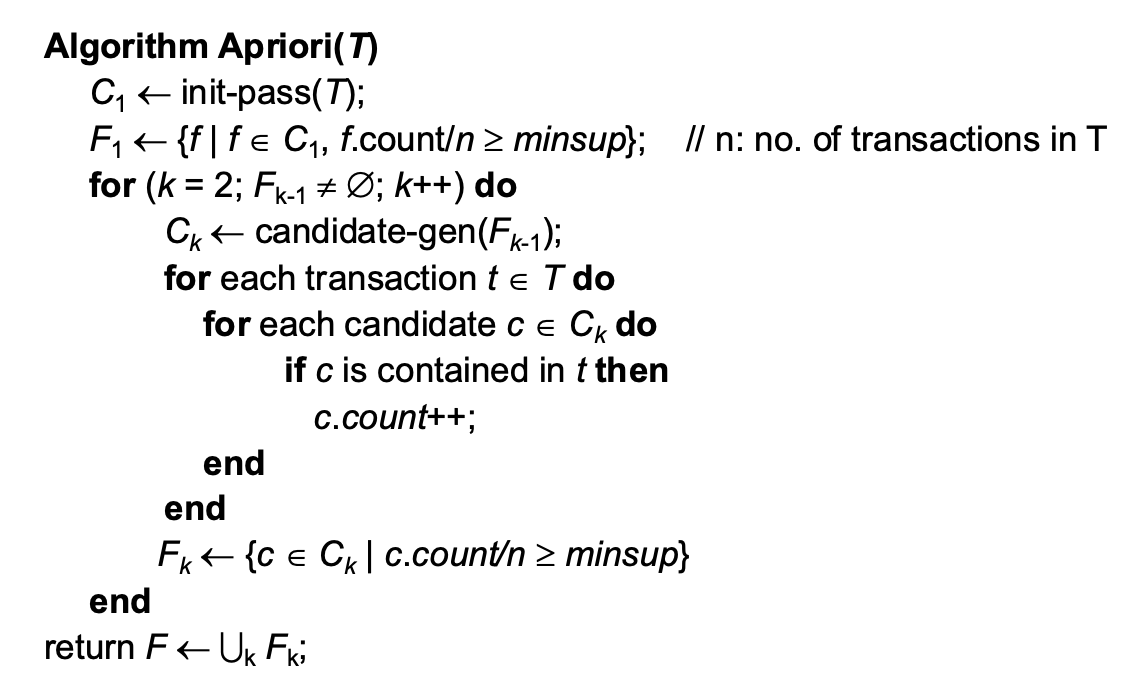
\includegraphics[width=0.8\textwidth]{Images/Apriori.png}
\end{figure}
\begin{figure}[H]
    \centering
    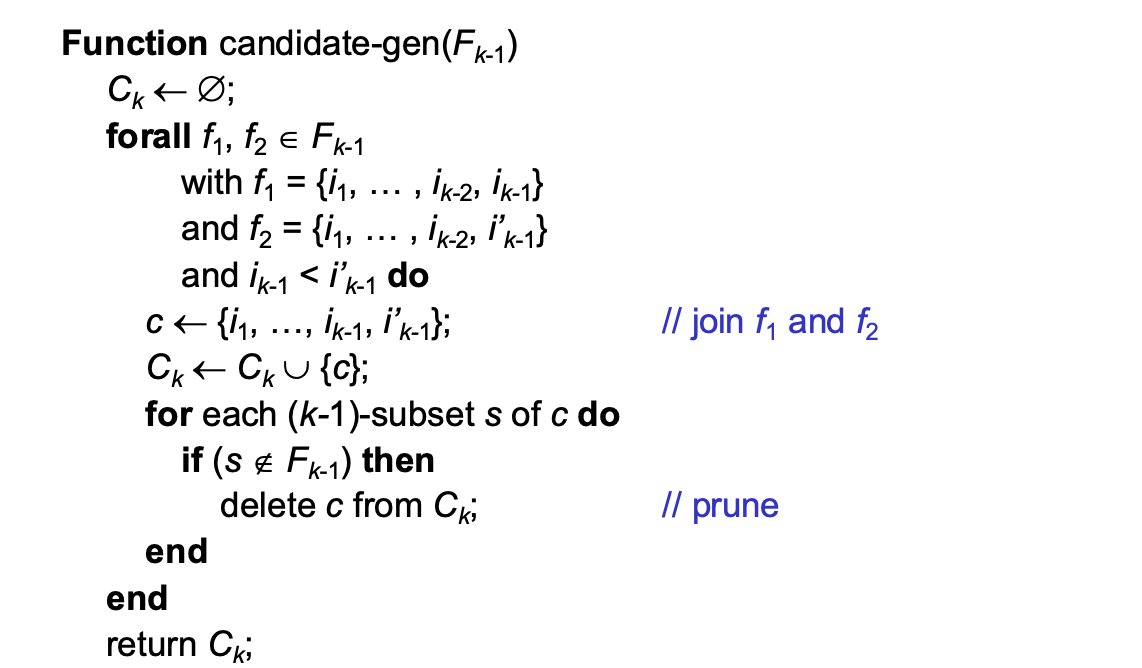
\includegraphics[width=0.8\textwidth]{Images/Candidate_gen_apriori.png}
\end{figure}

MS Apriori
\begin{figure}[H]
    \centering
    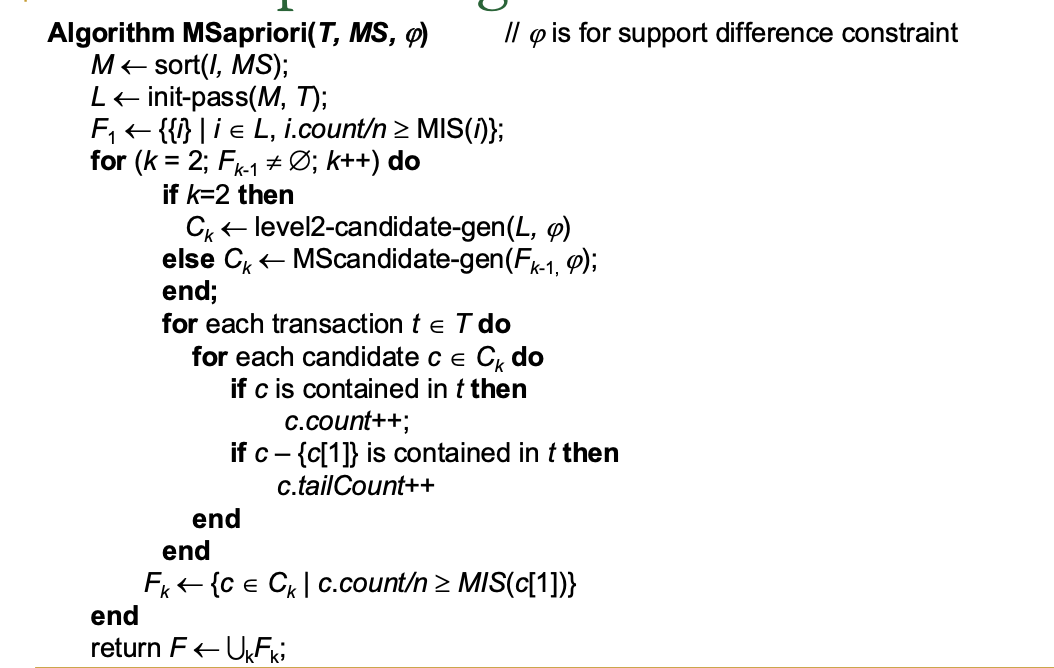
\includegraphics[width=0.8\textwidth]{Images/MsApriori.png}
\end{figure}
\begin{figure}[H]
    \centering
    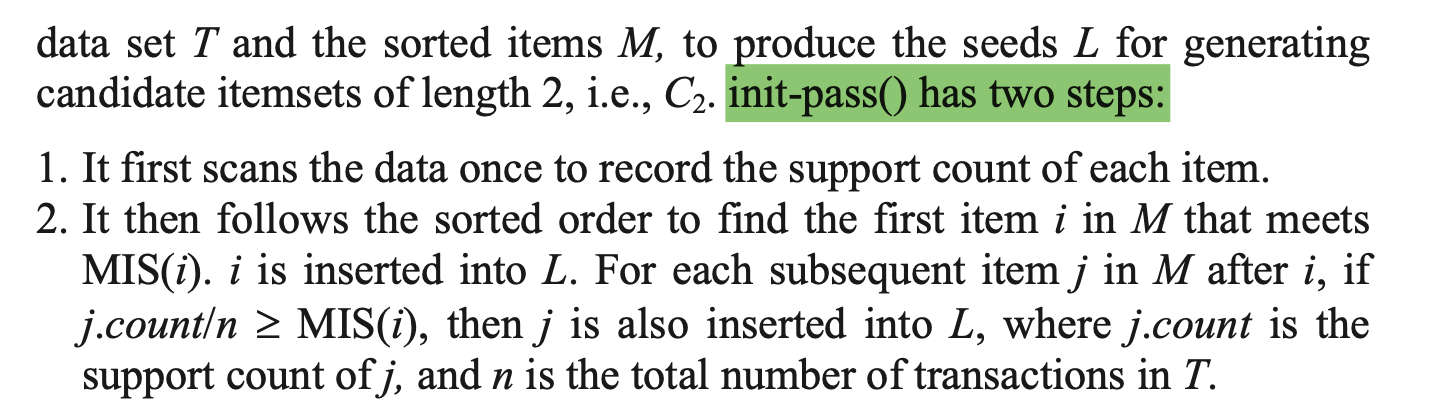
\includegraphics[width=0.8\textwidth]{Images/init_pass.png}
\end{figure}
\begin{figure}[H]
    \centering
    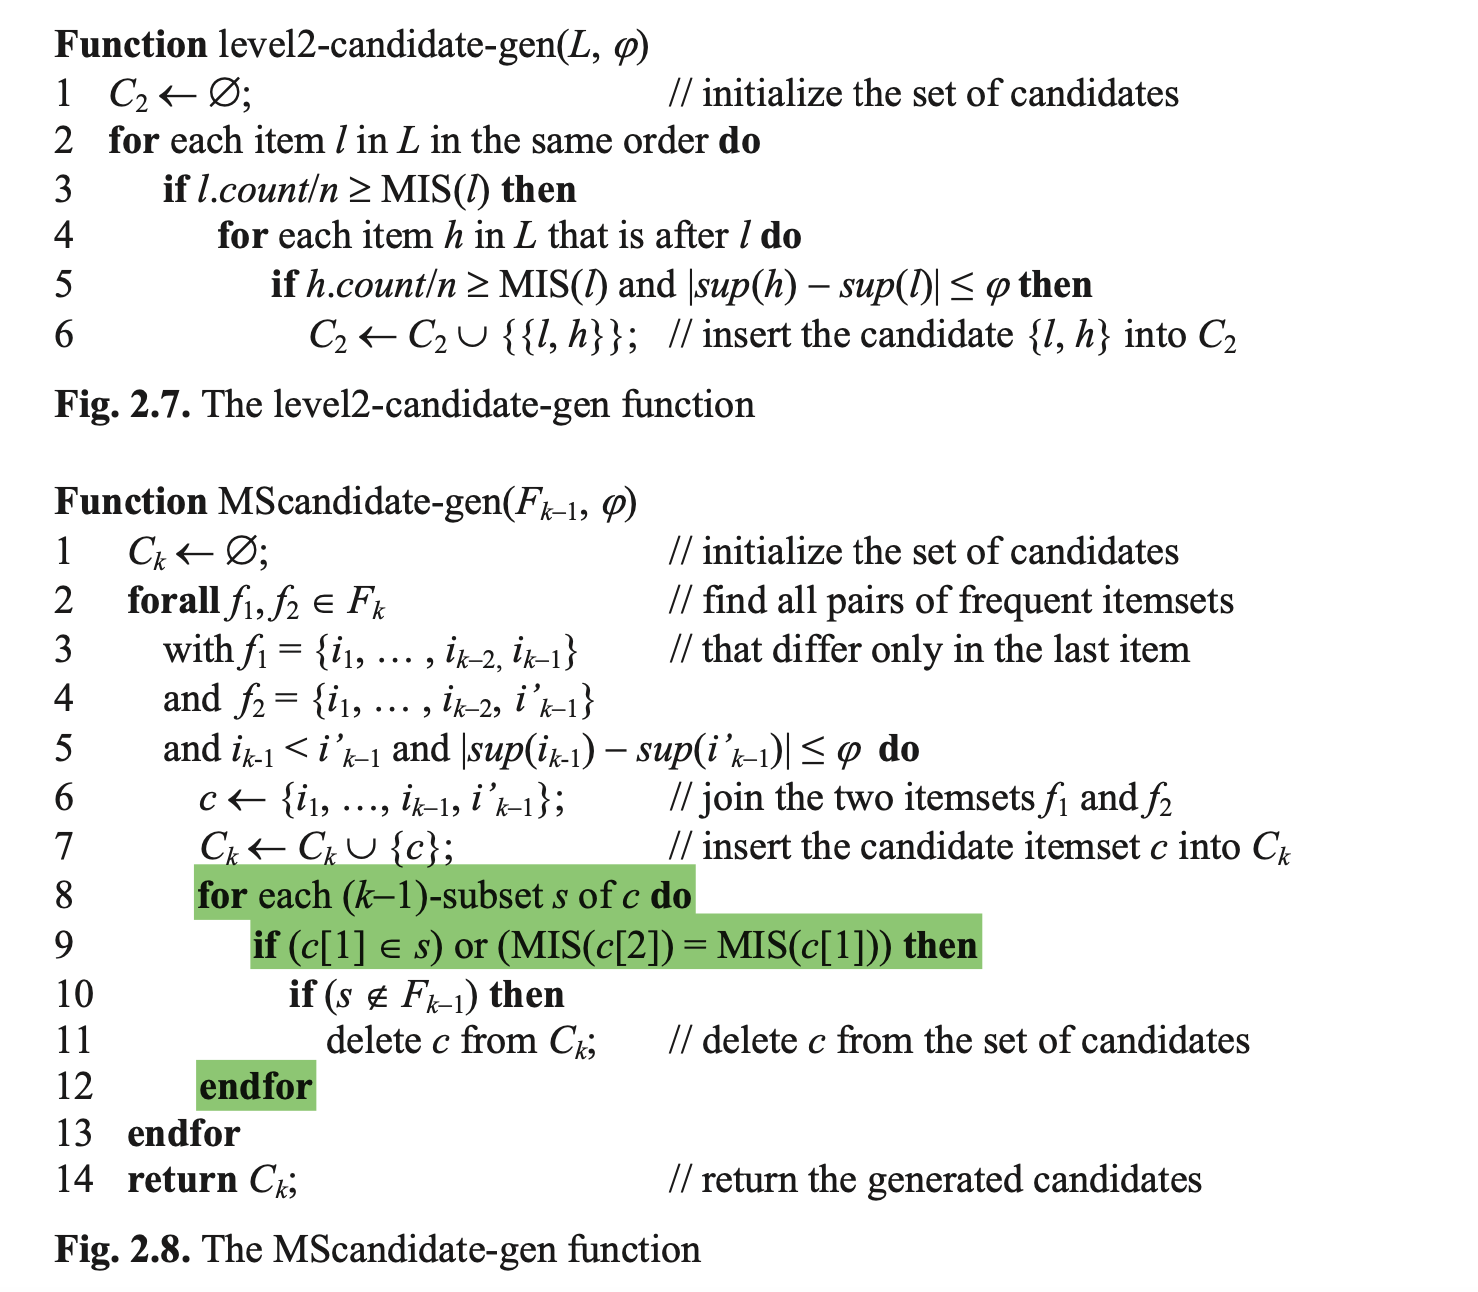
\includegraphics[width=0.8\textwidth]{Images/Candidate_gen_MS.png}
\end{figure}


\paragraph{Index for classificators}
\textbf{Precision} "Of the examples predicted as positive, how many are actually positive?"
\[
    \text{Precision} \, (p) = \frac{TP}{TP + FP}
\]

\textbf{Recall/sensitivity/true positive rate} "Of all the actual positive examples, how many did the model correctly identify?"
\[
    \text{Recall} \, (r) = \frac{TP}{TP + FN}
\]

index that combines precision and recall

\[
    F_1 = 2 \times \frac{p \times r}{p + r}
\]

\[
    \text{Sensitivity} = \frac{TP}{TP + FN}
\]

\textbf{Specificity/true negative rate}
\[
    \text{Specificity} = \frac{TN}{TN + FP}
\]

ROC: false positive rate on x axis, true positive rate on y axis



\paragraph{Entropy}
D is the dataset. C are the different classes in the dataset.

\[
    \text{entropy}(D) = - \sum_{j=1}^{|C|} \text{Pr}(C_j) \log_2 \text{Pr}(C_j)
\]

\[
    \text{entropy}_{A_i}(D) = \sum_{j=1}^{v} \frac{|D_j|}{|D|} \times \text{entropy}(D_j)
\]

\[
    \text{gain}(D, A_i) = \text{entropy}(D) - \text{entropy}_{A_i}(D)
\]

\paragraph{Naive based classification}
\[
    \text{Pr}(c \mid (a_1 \cdots a_n)) = \frac{\text{Pr}(c)  \text{Pr}((a_1 \cdots a_n) \mid c)}{\text{Pr}(a_1 \cdots a_n)}
\]
\[
    \text{Pr}(a_1 \cdots a_n) = \sum_{r=1}^{|C|} \text{Pr}(c) \text{Pr}((a_1  \cdots a_n) \mid c)
\]

\paragraph{Naive based text classification}
\[
    \text{Pr}(c_j \mid d_i, \hat{\Theta}) = \frac{\text{Pr}(c_j \mid \hat{\Theta}) \text{Pr}(d_i \mid c_j; \hat{\Theta})}{\text{Pr}(d_i \mid \hat{\Theta})}
\]
\[
    = \frac{\text{Pr}(c_j \mid \hat{\Theta}) \prod_{k=1}^{|d_i|} \text{Pr}(w_{d_i,k} \mid c_j; \hat{\Theta})}{\sum_{r=1}^{|C|} \text{Pr}(c_r \mid \hat{\Theta}) \prod_{k=1}^{|d_i|} \text{Pr}(w_{d_i,k} \mid c_r; \hat{\Theta})}
\]

This is the probability of each class in the training set
\[
    \text{Pr}(c_j \mid \hat{\Theta}) = \frac{1}{|D|} \sum_{i=1}^{|D|} \text{Pr}(c_j \mid d_i)
\]
This is the probability of the class c with the parameters tetha generating the document d. This depends on the probability of generating a document of length d, the possible ways of rearranging the words in the document (factorial term), the number of times the word t is in the document d and the probability of the word being generated by the class with parameters tetha.
\[
    \text{Pr}(d_i \mid c_j; \Theta) = \text{Pr}(|d_i|) \cdot |d_i|! \prod_{t=1}^{|V|} \frac{\text{Pr}(w_t \mid c_j; \Theta)^{N_{ti}}}{N_{ti}!}
\]
This is the probability of a word being generated by a class. This is at the numerator the summations on the whole set of documents of the number of times the word appears in a document multiplied per the probability of the document of being of class c.
At the denominator we sum the same probability for all the word in the dataset.
\[
    \text{Pr}(w_t \mid c_j; \hat{\Theta}) = \frac{\sum_{i=1}^{|D|} N_{ti} \text{Pr}(c_j \mid d_i)}{\sum_{s=1}^{|V|} \sum_{i=1}^{|D|} N_{si} \text{Pr}(c_j \mid d_i)}
\]

\[
    \text{Pr}(d_i \mid \hat{\Theta}) = \sum_{r=1}^{|C|} \text{Pr}(c_r \mid \hat{\Theta}) \text{Pr}(d_i \mid c_j; \Theta)
\]

\section{SVMs}
Krun Tucker conditions

\[
    \frac{\partial L_p}{\partial w_j} = w_j - \sum_{i=1}^{r} y_i \alpha_i x_{i,j} = 0, \quad j = 1, 2, ..., m
\]

\[
    \frac{\partial L_p}{\partial b} = - \sum_{i=1}^{r} y_i \alpha_i = 0
\]

\[
    y_i \left( \langle w, x_i \rangle + b \right) \geq 1, \quad i = 1, 2, ..., r
\]

\[
    \alpha_i \geq 0, \quad i = 1, 2, ..., r
\]

\[
    \alpha_i \left( y_i \left( \langle w, x_i \rangle + b \right) - 1 \right) = 0, \quad i = 1, 2, ..., r
\]

Wolfe dual
\[
    L_D = \sum_{i=1}^{r} \alpha_i - \frac{1}{2} \sum_{i=1}^{r} \sum_{j=1}^{r} y_i y_j \alpha_i \alpha_j \langle x_i, x_j \rangle
\]

\[
    \text{Subject to:} \quad \sum_{i=1}^{r} y_i \alpha_i = 0
\]

\[
    \alpha_i \geq 0, \quad i = 1, 2, ..., r
\]

The linear separator
\[
    \langle w, x \rangle + b = \sum_{i \in SV} y_i \alpha_i \langle x_i, x \rangle + b = 0
\]


Soft margin
\[
    \frac{\partial L_p}{\partial w_j} = w_j - \sum_{i=1}^{r} y_i \alpha_i x_{i,j} = 0, \quad j = 1, 2, ..., m
\]

\[
    \frac{\partial L_p}{\partial b} = - \sum_{i=1}^{r} y_i \alpha_i = 0
\]

\[
    \frac{\partial L_p}{\partial \xi_i} = C - \alpha_i - \mu_i = 0, \quad i = 1, 2, ..., r
\]

\[
    y_i \left( \langle w, x_i \rangle + b \right) - 1 + \xi_i \geq 0, \quad i = 1, 2, ..., r
\]

\[
    \xi_i \geq 0, \quad i = 1, 2, ..., r
\]

\[
    \alpha_i \geq 0, \quad i = 1, 2, ..., r
\]

\[
    \mu_i \geq 0, \quad i = 1, 2, ..., r
\]

\[
    \alpha_i \left( y_i \left( \langle w, x_i \rangle + b \right) - 1 + \xi_i \right) = 0, \quad i = 1, 2, ..., r
\]

\[
    \mu_i \xi_i = 0, \quad i = 1, 2, ..., r
\]

\[
    \text{Maximize: } L_D(\alpha) = \sum_{i=1}^{r} \alpha_i - \frac{1}{2} \sum_{i=1}^{r} \sum_{j=1}^{r} y_i y_j \alpha_i \alpha_j \langle x_i, x_j \rangle
\]

\[
    \text{Subject to:} \quad \sum_{i=1}^{r} y_i \alpha_i = 0
\]

\[
    0 \leq \alpha_i \leq C, \quad i = 1, 2, ..., r
\]

\end{document}